\section{Resolución}

Tenemos $k$ calles bidireccionales a comparar y buscamos de entre ellas la que minimice el valor del camino más corto entre $s$ y $t$ luego de construirla. Este problema puede ser modelado con un digrafo, donde todo par de puntos está conectado por a lo sumo una arista dirigida. Luego, $s$ y $t$ contarán, o no, con un camino mínimo original el cual buscamos mejorar, o crear, agregando las aristas correspondientes a las calles bidireccionales propuestas. Proponemos entonces el siguiente algoritmo:

\begin{enumerate}
    \item Armamos un digrafo que modele a la ciudad, donde cada punto es un nodo y cada calle unidireccional es una arista. 
    \item Utilizamos el algoritmo de Dijkstra para encontrar los caminos minimos desde $s$ hacia todos los nodos.
    \item Dando vuelta las aristas, utilizamos el algoritmo de Dijkstra para encontrar el camino mínimo de todos los nodos hacia $t$ en el digrafo original.
    \item Por cada arista bidireccional $k_i$ de largo $l(k_i)$ que une a dos puntos $v$ y $w$, y sea $d(u,p)$ la longitud del camino más corto entre los vértices $u$ y $p$, comparamos el mínimo de entre: 
    \begin{itemize}
        \item[--] La longitud del mejor camino hasta ahora entre $s$ y $t$.
        \item[--] Ir desde $s$ hasta $v$, viajar a $w$ y desde $w$ hasta $t$ con costo $d(s,v) + l(k_i) + d(w,t)$.
        \item[--] Ir desde $s$ hasta $w$, viajar a $v$ y desde $v$ hasta $t$ con costo $d(s,w) + l(k_i) + d(v,t)$.
    \end{itemize}
    \item Devolver la longitud mínima de entre todas las halladas.
\end{enumerate}

La idea detrás del mismo es agrupar a todas las oficinas en $W$ conjuntos disjuntos, los cuales dispondrán de un módem cada uno. De esta forma, cada oficina tendrá acceso a exáctamente un módem. Puede demostrarse que en una solución minimal, ninguna oficina puede estár conectada a más de uno. Luego, aplicando el algoritmo de Kruskal, se pueden hallar las $W$ componentes conexas tal que minimicen los costos de los cables y así obtener la solución al problema. 

\vspace{1em}

\subsection{Demostración de Correctitud}
\vspace{1em}

Primero vamos a observar que en una solución minimal no puede haber más de $W$ árboles en el bosque. Esto se debe a que, como tenemos $W$ módems, no tendríamos un módem por árbol, por lo que habría al menos un árbol de oficinas que quedaría sin conexión. 

\vspace{1em}

Luego queremos probar que en una solución que minimiza los costos de los cables no puede haber menos de $W$ árboles. Para lograrlo, asumimos que existe una solución mínima tal que se cumple que las oficinas están repartidas en menos de $W$ conjuntos conexos. Podríamos entonces darle un módem a alguna oficina de cada árbol, de esta manera todas las oficinas tendrían conexión. Como tenemos menos de $W$ árboles, nos sobrarían módems, entonces, si elegimos una oficina ``hoja", es decir que tenga una sola arista, y le asignamos uno de los módems que nos sobraron, estaríamos recortando costos ya que podríamos eliminar la conexión que esta oficina tenía previamente. Por lo que llegamos a un absurdo, concluyendo que la asumpción de que teníamos una solución minimal es falsa.

\vspace{1em}

De esta manera probamos que en una solución minimal la cantidad de árboles no es mayor ni menor a $W$, por lo que notamos que debe ser exactamente $W$. 

\vspace{1em}

Encontrar las $W$ componentes conexas tal que minimicen los costos se puede lograr siguiendo el invariante del algoritmo de Kruskal. Esto es porque luego de $i$ pasos de Kruskal, tendremos $N - i$ componentes conexas, tal que no existe otro bosque de $i$ aristas que sume a un costo menor. Entonces, luego de realizar $N - W$ pasos, tendremos $N - (N - W) = W$ conjuntos disjuntos de oficinas, conectadas entre sí minimizando los costos. 

\vspace{1em}

Queda entonces demostrado que el algoritmo planteado es correcto ya que demostramos que para hallar una solución que minimice los costos es necesario dividir a las oficinas en exactamente $W$ componentes conexas y aprovechamos el algoritmo de Kruskal que nos ofrece una manera de encontrar dicha división.

\vspace{1em}

\subsection{Implementación}
\vspace{1em}

Presentamos a continuación una posible implmentación de la solución explicada:

\lstinputlisting[mathescape=true, language=pseudo, label=e, caption={Pseudocódigo}]{ej3.pseudo}


\subsection{Análisis de la Complejidad}
\vspace{1em}


La complejidad del algoritmo presentado es la siguiente: 

\begin{itemize}
    \item Obtener input \qquad \qquad \qquad \quad $\rightarrow O(n)$
    \item Generar grafo completo \qquad \quad $\rightarrow O(n^2)$
    \item Ordenar aristas con QuickSort $\rightarrow O(n^2 log(n^2))$
    \item Algoritmo de Kruskal \qquad \qquad $\rightarrow O(n^2 \alpha(n))$
\end{itemize}

Sabemos que $\alpha(n)$ crece más lentamente que $log(n)$ por lo que la complejidad total del algoritmo es $O(n^2 log(n^2))$.

\vspace{1em}

Una posible optimización al algoritmo, observando que la parte computacionalmente más costosa de este es aplicar QuickSort, es aplicar BucketSort agrupando las aristas por peso de la siguiente manera.

\vspace{1em}

Aprovechando las restricciones de los parámetros del enunciado, notamos que la distancia máxima entre dos vértices es $\sim30000$. Esta se da cuando uno de los vértices se ubica en una esquina del rango posible y el otro en la esquina opuesta. Por ejemplo, $x_1 = (-10000, \ -10000) \ \wedge \  x_2 = (10000, \ 10000)$.

\vspace{1em}

Agrupamos las aristas de la siguiente forma. Inicialmente, elegimos un número arbitrario llamado $k$, y generamos un vector de $30000 / k$ posiciones de tal forma que en la posición $i$-ésima del vector ubicamos las aristas que tienen una distancia que pertenecen al rango $[k \cdot i, \ k \cdot (i+1))$. Como la distancia esta acotada por 30000 y cada rango es disjunto, sabemos que cada arista estará ubicada en exactamente uno de los rangos posibles. Nosotros elegimos $k = 100$ arbitrariamente.

\vspace{1em}

Agrupando las aristas de esta manera, sabemos que para toda arista que se halla en el $i$-ésimo bucket, su peso será menor al de cualquiera de los buckets mayores a $i$.

\vspace{1em}

Luego ordenamos las aristas de la primer posición del vector y empezamos a aplicar Kruskal con las primeras aristas ordenadas. Cuando ya analizamos todas las de la primer posición, ordenamos las de la segunda posición y seguimos aplicando kruskal, así sucesivamente hasta acabar con el algoritmo. De esta manera, nos evitamos ordenar la mayoría de las aristas del grafo.

\vspace{1em}

Cabe aclarar que esta optimización no mejora la complejidad del algoritmo pero, en la práctica, si mejora considerablemente la constante. 

\vspace{1em}
Para medir los tiempos de cómputo, por cada $N \in [100, 200,..., 2000]$ generamos 100 tests aleatorios y calculamos el promedio del tiempo de ejecución de estos. Como se puede apreciar en el gráfico, a medida que se aumenta el tamaño del input, el algoritmo crece de la forma mencionada, aunque BucketSort tiene una curva de crecimiento más baja.\footnote{Todos los tests fueron ejecutados desde el mismo ordenador para todos los algoritmos, con un CPU Intel Core i5 6400 (4-core) y 16gb de RAM DDR4 (1066MHz).}


% \begin{figure}[h]
%     % \ContinuedFloat
%     \centering
%     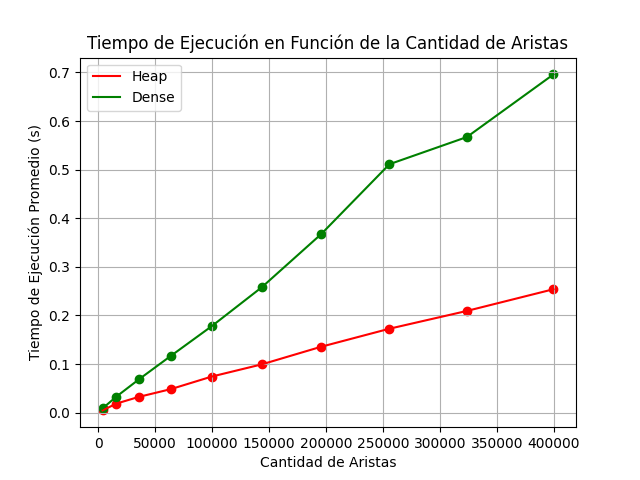
\includegraphics[width=0.7\textwidth, trim=0 0 0 10]{./grafico.png}
%     \label{grafico}
% \end{figure}

\newpage
\subsection{Implementaciones de Kruskal}
\vspace{1em}

Observando que el verdadero costo computacional de nuestro algoritmo proviene de realizar Kruskal (y el correspondiente ordenamiento de las aristas), podemos experimentar con diferentes implementaciones y optimizaciones del mismo para buscar una mayor eficiencia. En nuestra versión original del algoritmo realizamos un Kruskal con un DSU semi-optimizado con Path Compression, pero existen más formas de mejorarlo. En esta sección, nos dedicaremos a analizar y comparar los tiempos de ejecución de diferentes implementaciones para entradas de tamaños variados.

\vspace{1em}
Comencemos explicando cuáles son las diferentes optimizaciones posibles del DSU. El \textit{Disjoint Set Union} es la estructura de datos que le permite al algoritmo de Kruskal unir las diferentes componentes conexas de nuestro grafo en forma eficiente. Ésta cuenta con dos operaciones: \textbf{find()}, que dado un elemento devuelve el conjunto al que pertenece, y \textbf{unite()}, que dados dos conjuntos diferentes los une. 

\vspace{1em}
En particular, hay dos posibles optimizaciones para el DSU. El ya mencionado \textit{Path Compression} es una mejora a la función de \textbf{find()}, donde en vez de recorrer varios elementos del conjunto hasta llegar al representante del mismo se devuelve el representante directamente, comprimiendo de esta forma el camino recorrido. Por otro lado, \textit{Union by Rank} es una optimización de la función \textbf{unite()}, donde al unir dos conjuntos buscamos que el de menor cardinal se acople al de mayor, logrando que se modifiquen la menor cantidad de referencias posibles. Esto puede lograrse almacenando el tamaño de cada conjunto en un vector aparte y operando en él en tiempo constante.

\vspace{1em}
Por otro lado, podemos comparar tiempos de ejecución con una implementación de Kruskal optimizada para grafos densos, donde si se tienen $n$ vértices y $m$ aristas, se da que $m \sim n^2$. Ésta versión del algoritmo no utiliza una estructura de DSU sino más bien una matriz de adyacencias, y no requiere de ordenar las aristas. Puede demostrarse que la complejidad de ésta implementación es O($n^2$), mejor al O($n^2 * log(n^2)$) = O($n^2 * log(n)$) de Kruskal con DSU. Por cómo funciona nuestra solución, el grafo que modela el problema de los modems es uno completo, con lo cual se esperaría que ésta implementación para grafos densos sea más rápida.

\vspace{1em}
Para esta experimentación comparamos los tiempos de ejecución de las tres implementaciones del algoritmo de Kruskal (DSU sin y con optimizaciones, y para grafos densos) con casos de test random generados en Python. Se consideraron la cantidad de oficinas $N \in [100, 200,..., 1000]$, y para cada $N$ diferente se generaron 100 test al azar respetando las restricciones del enunciado original. De este modo, se tomó el promedio de los runtime para cada tamaño de entrada diferente y graficamos las curvas de cada algoritmo en el siguiente cuadro\footnote{Los tests fueron ejecutados desde el mismo ordenador para todos los algoritmos, con un CPU Intel Core i5 6400 (4-core) y 16gb de RAM DDR4 (1066MHz).}:

% \begin{figure}[h]
%     %\ContinuedFloat
%     \centering
%     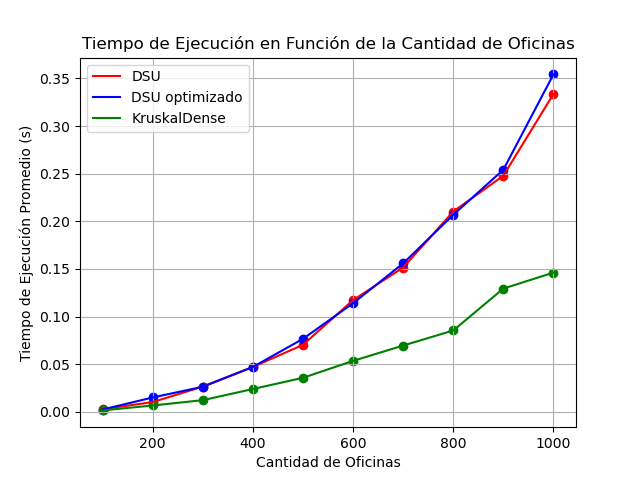
\includegraphics[width=0.7\textwidth, trim=0 0 0 10]{./graficoKlinear.png}
%     \caption{Tiempos de ejecución de las distintas implementaciones de Kruskal con entradas random.} \label{graficoImplementaciones}
% \end{figure}

\vspace{1em}
Como se puede apreciar en el gráfico, la implementación optimizada para grafos densos es drásticamente más rápida, en promedio dos veces mejor que las otras dos (esto aumentaría a mayor tamaño de entrada). Ésto verifica lo previamente estimado y muestra que esta versión del algoritmo es la mejor elección de entre las tres para este problema particular. Por otro lado, podemos ver que no hay mucha diferencia en tiempos de ejecución entre ambas implementaciones con DSU. Mientras que claramente la implementación para grafos densos de Kruskal es la más rápida, utilizar un DSU básico u optimizado no hace diferencias notables en tiempos de ejecución. Esto podría deberse a que la complejidad dominante del algoritmo es el ordenamiento, muy superior a la de las operaciones del DSU. Luego, podría ser que a causa de la variación en la velocidad del ordenamiento (en nuestro caso QuickSort) no se pueden apreciar mejoras entre ambas versiones. Creemos que, en teoría, aumentando considerablemente la cantidad de tests cases por cada tamaño de entrada $N$ diferente, eventualmente se reduciría esta variación, permitiendo ver una mejora en tiempos de ejecución del DSU optimizado. 